\chapter{Background and Related Work (20)}
\label{chp:background}
%%%%%%%%%%%%%%%%%%%%%%%%%%%%%%%%%%%%%%%%%%%%%%%%%%%%%%%%%%%%%%%%%%%%%%%%%%
\section{Container Terminal Operations} 
%%%%%%%%%%%%%%%%%%%%%%%%%%%%%%%%%%%%%%%%%%%%%%%%%%%%%%%%%%%%%%%%%%%
Container terminals represent critical nodes within global supply chains and facilitate the transition between maritime and Hinterland transportation networks. [seaport erläuterung!] They serve as interfaces between deep-sea vessels and hinterland transportation systems including road, rail, and inland waterway transport. Modern container vessels have a capacity of more than 20,000 containers in a single voyage, requiring container terminals to process large cargo volumes efficiently while maintaining short turnaround times and high service quality [SOURCE]. Since their introduction in the 1960s, standardized containers have become the dominant unit for global freight transportation. To ensure comparability across different container sizes, container throughput is commonly measured in Twenty-foot Equivalent Units (TEU). A standard 20-foot container corresponds to one TEU, whereas a 40-foot container corresponds to two TEUs \cite{Hartmann2005cenariosforCTSimulation}. Container terminals operate under considerable operational pressure. Increasing international trade volumes, larger vessels, and growing demands for rapid cargo handling require terminal operators to coordinate numerous interdependent processes and resources simultaneously. As a result, operational decisions directly affect vessel berth times, truck turnaround times, a terminals throughput, and overall service quality \cite{CTSteenken2004,OptimizingCTs2023}. The empirical context of this thesis is the HHLA Container Terminal Burchardkai (CTB) located in the Port of Hamburg. The CTB is the largest container terminal in Hamburg and. The terminal handles large volumes of import, export, and transshipment containers while coordinating interactions between vessels, trucks, rail services, storage yards, and container handling equipment. [ACTUAL NUMBERS] 6.3 mio HHLA total 
[Abbildung Hinterland/ Wasserseite Abgrezung Bild von der HHLA]

\subsection{Container Terminals as Complex Logistics Systems} 
Container terminals are handled  as highly complex logistics systems due to the large number of interacting resources, transportation modes, and operational dependencies involved in the everyday operations.  \cite{CTSteenken2004,OptimizingCTs2023}. 

\subsubsection{Container Flows} 
Within a seaport container terminal, containers move between multiple transportation modes and storage locations. A container may arrive by deep-sea vessel, feeder vessel, truck, or rail and subsequently leave the terminal using any of these transport modes. [HINTERLAND ERWÄHNEN] Consequently, a terminal continuously coordinates container flows between the seaside and the landside of the supply chain \cite{Hartmann2005cenariosforCTSimulation}.  Hartmann distinguishes four primary transportation modes within container terminal operations: deep-sea vessels, feeder vessels, trucks, and rail services. Together, these modes create numerous possible transport paths through the terminal and generate highly dynamic container flows that must be coordinated efficiently \cite{Hartmann2005cenariosforCTSimulation}. Most containers entering a terminal undergo at least one temporary storage phase within the container yard before being transferred to their outbound transportation mode. Therefore, terminal operations must coordinate not only transportation processes but also inventory management and storage allocation decisions \cite{CTSteenken2004}. 
Figure: Container Flow through a Container Terminal  [Wasserseite -> LAGER -> hINTERLAND Günstig in Bezug auf Hamburger Ladungsverteilung]

\subsubsection{Yard Components and Resources}
Container terminals consist of multiple operational subsystems that interact continuously. Bett et al. distinguish three primary terminal areas: the quayside, the yard area, and the landside. The quayside includes berths and quay cranes used for vessel loading and unloading. The yard acts as an intermediate storage area for containers, while the landside connects the terminal to trucks and rail operations\cite{Bett2024}. For this Thesis relevant is the terminals yard area, that splits into three seperate areas in the case of the CTB in Hamburg:

\begin{enumerate}
    \item \textbf{Automatic storage Blocks:} The majority of containers is stored in the automatic storage blocks, operated by "Rail Mounted Gantry Cranes" - therefore often called RMG-Blocks. The CTB operates 22 RMG-Blocks with a total capacity of 2231 operative TEU slots and 3 RMGs per Block, operating between the waterside and the landside.[total of 40.000 operative TEU in Block]  up to 5 high due to operational moves. 

    \item \textbf{Manual Yard:} In addition to the automated storage area, containers can be stored in the manually operated yard. Due to its central location within the terminal, this area is frequently used for operationally flexible storage depending on the assigned vessel berth, yard workload, and equipment availability. Container movements are typically performed by manually operated handling equipment.

    \item \textbf{Empty Container Yard:} Empty containers are primarily stored in a dedicated empty container yard. Unlike full containers, empty containers are generally not assigned to a specific customer order but are managed as interchangeable inventory within a shipping line's container fleet. 
    We want containers whose auslieferung noz numerical is, we want to stroe them as dense as possible, different handling equipment, and up to 6 high. 
    Storing empty containers separately prevents them from occupying or being stacked on top of storage positions of full containers that are linked to specific transport orders. The empty container yard is operated using reach stackers, allowing storage heights of up to six containers.
    
\end{enumerate}
hhla wEBSEITE bILD VOM bURCHARDKAI 


Trucks can be ordered to pick up and deliver their cargo at all of these yard sections, waiting in transfer points to be operated by the respective resources. Resource shortages or inefficiencies within one subsystem often show effects throughout the whole terminal and negatively impact other operations \cite{CTSteenken2004}.

\subsubsection{Interdependencies Between Terminal Processes}
An important characteristic of container terminals is the strong interdependency of their operational processes. Individual decisions rarely affect only one subsystem. Instead, local disturbances often propagate throughout the entire terminal. [For example, delayed vessel arrivals may postpone container unloading operations, which subsequently affects yard occupancy levels. Increased yard congestion can reduce crane productivity and generate longer waiting times for trucks arriving at the terminal. These delays may ultimately result in congestion at terminal gates and reduced service quality for trucking companies] - Mit Fokus, was bedeutet das eigentlich tatsächlich für ein terminal? \cite{CTSteenken2004,Bett2024}. The complexity of these interactions is one of the primary reasons why analytical optimization approaches alone are often insufficient for evaluating operational decisions in container terminals. 

\subsection{Truck Handling Processes} 
\subsubsection{Importance of Truck Operations} 
Road transportation is a major component of hinterland connectivity in modern container terminals.  As a consequence, terminals must coordinate large numbers of truck arrivals while maintaining acceptable service levels and avoiding excessive congestion and effects on public traffic in the port area \cite{CTSteenken2004,CTprocessMiningTAS2020}. Fluctuating truck arrival patterns can exceed the available processing capacity of gates, yard equipment, and storage areas, resulting in longer waiting times and reduced terminal efficiency \cite{Bett2024,CTprocessMiningTAS2020}. 

\subsubsection{A [Typical] Truck Visit Process} 
To regulate truck arrivals and reduce congestion, many container terminals employ a Truck Appointment System (TAS). [Thats importnant as a decsion support resulting tool!] Within a TAS, trucking companies reserve a predefined time slot before visiting the terminal and specify the container transactions that will be executed during the visit \cite{Bett2024,CTprocessMiningTAS2020}. A typical truck visit begins with the reservation of an appointment slot and the submission of the corresponding transport order. When arriving at the terminal, the truck passes through an automated pre-gate area where Optical Character Recognition (OCR) systems identify containers, vehicle registration plates, and aggregates touring information with booking information. [Despite the hourly booking slots, the Depending on the current workload and gate queue lengths, the truck may have  Referr to Poisson later in the arrival distribution section]to wait before being processed at the physical gate and officially entering the terminal area \cite{Bett2024}. After entering the terminal, the truck drives to the assigned container yard location. Depending on the transport order, the truck can perform one or multiple container transactions. These transactions may include: 

\begin{itemize}
    \item delivering an export container, 
    \item receiving an import container, 
    \item delivering or receiving  multiple containers while at the same yard location, 
\end{itemize} 

A particularly efficient operational pattern is referred to as a \textit{multi move}. In a multi move, a truck delivers one or more export containers and subsequently picks up one or more import containers during the same terminal visit. Multi moves reduce empty truck trips, improve truck utilization, lower emissions, and decrease congestion both inside and outside the terminal, but require efficient routing by the terminal \cite{CTprocessMiningTAS2020}. Following the completion of all assigned transactions, the truck proceeds to the exit gate, completes the required departure procedures, and leaves the terminal. The total time spent between entering and leaving the terminal is commonly referred to as the \textit{Truck Turnaround Time (TTT)}, which represents one of the most important performance indicators in truck and overall terminal operations \cite{Bett2024}. 

\subsubsection{Terminal Operating Systems}
Modern container terminals rely on integrated information systems to coordinate operational activities. At the center of these systems are the Order Management and Terminal Control System (TCS), that orchestrate the movements and storage of containers across terminal subsystems and manages operational orders throughout the terminal lifecycle. The TOS is typically connected to specialized subsystems including a Gate Operating Systems (GOS), Yard Management Systems, Equipment Control Systems, and appointment management platforms. Together, these systems continuously generate and manage operational event data whenever trucks arrive, containers are handled, orders are updated, or terminal resources execute work instructions. Each subsystem stores a different subset of operational information. While gate systems primarily record arrival and departure events and details, yard management systems capture container movements, assign storage locations and and communicates with the equipment control system thats responsible for the equipment execution orders. Consequently, the complete reconstruction of truck visits often requires the integration of multiple operational data sources. For the purposes of this thesis, the Order and Terminal Control System serves as the primary data source. Additional information from other operational systems is subsequently used to enrich and validate the resulting event log. The employed data integration process is described in detail in Chapter~\ref{chp:experiments_and_framework}. 

\subsubsection{Sources of Operational Delays} 
Truck turnaround times are influenced by various operational factors that function individually or interdependent throughout the terminal processes. Common reasons for delay include:

\begin{itemize} 
    \item congestion at entry and exit gates, also caused and affected by road traffic outside the terminal
    \item pick up containers that are buried due to unexpected long dwell time on the terminal
    \item truck traffic congestion within container yard sections and main routes,
    \item limited availability of container handling equipment (CHE), 
    \item high occupancy levels within storage blocks, 
    \item resource and priority conflicts between truck and vessel operations, 
    \item unexpected equipment failures or maintenance activities 
\end{itemize} 

Because these factors are highly interdependent, local disruptions often affect the entire terminal operations. For example, insufficient yard crane availability and a prioritised vessel departure in time can increase truck service time, which affects the trucks waiting times in the yard, which subsequently results in traffic congestion on the terminal area, a lower gate throughput and overall slowed Hinterland performance \cite{CTSteenken2004,Bett2024}. 

\subsubsection{Operational Performance Indicators} 
The performance of truck operations is commonly evaluated using a set of operational key performance indicators (KPIs). 
\begin{itemize} 
    \item \textbf{Truck Turnaround Time (TTT):} Total time a truck spends inside the terminal between entry and exit. 
    \item \textbf{Waiting Time:} Time spent waiting for gate processing, yard equipment, or storage area access.  
    \item \textbf{Yard Utilization:} Degree to which storage areas are occupied and operational resources are utilized.
\end{itemize} 

Among these indicators, Truck Turnaround Time is frequently considered the most important measure of truck service quality because it directly reflects the operational efficiency experienced by trucking companies and cargo owners and is therefore one out of four main KPIS for the HHLA Container Terminals.\cite{Bett2024,CTprocessMiningTAS2020}.

\subsection{Simulation-Based Decision Support in Container Terminals} 
\textit{This is now trying to explain Why is there a need for better decision support in container terminals in general, why is simulation a common approach for that purpose, and why are traditional simulation approaches insufficient?}

The Management of Container Terminals continuously faces operational decision making challenges. Decisions regarding truck appointment policies, resource allocation, equipment scheduling, maintenance planning, and yard management need to be made while operations remain active. Because container terminal processes are very interconnected, local decisions can quickly affect other parts of the system and influence waiting times, resource utilization, throughput, and eventually customer service quality.
Although terminal managers often possess extensive operational experience, many decisions involve considerable uncertainty. Changes to operational procedures or capacity allocations may have unintended consequences, create congestion, increase handling times, or reduce service reliability. As a result, decision-making in container terminals increasingly relies on analytical and digital decision-support approaches that allow operational alternatives to be assessed before implementation. Simulation as a decision support tool in container terminal management has become an interesting and widely adopted research field. The application is reality is still lacking though, due to high complexity, costs, and a missing technical expertise or priority in the terminal teams. Running a Simulation enables managers and researchers to evaluate operational scenarios in a virtual environment without affecting live terminal operations. By reproducing the interactions between trucks, handling equipment, storage areas, and gate processes, simulation can estimate the effects of operational changes before they are implemented in practice. Typical applications of simulation in container terminals include the evaluation of Truck Appointment Systems (TAS), equipment allocation strategies, resource planning, yard management and storage placement strategies. Simulation is especially valuable when analysing congestion effects, resource bottlenecks, and operational trade-offs that are difficult to evaluate based on purely critical analytical thinking. A variety of studies have demonstrated the usefulness of simulation for improving truck turnaround times, resource utilization, and overall terminal performance \cite{Kastner2021,Bett2024,Carboni2025}. 

\begin{sloppypar}
Various simulation paradigms have been applied in terminal research. Discrete Event Simulation (DES) is the most frequently used approach because container terminal operations can naturally be represented as sequences of discrete operational events such as truck arrivals, gate processing, container handling, and equipment usage. Other approaches such as System Dynamics, Agent-Based Modeling, and microscopic traffic simulation have also been applied to investigate specific operational and strategic questions \cite{Muravev2019,Muravev2021,Carboni2025}. A more detailed discussion of simulation methodologies is provided in Section~2.3. Despite their widespread adoption, traditional simulation projects suffer from several limitations. Developing a simulation model typically requires extensive domain knowledge, detailed process understanding, and considerable modeling effort. The collection, formalization, implementation, calibration, and validation of process knowledge often represent the most time-consuming phases of a simulation project. Furthermore, manually developed simulation models most of the time rely on expert assumptions regarding process behavior. However, experts often describe how processes are intended to operate rather than how they are actually executed in practice, therefore, unintended discrepancies can appear between the simulation model and the real operational processes \cite{PMRozinat2009}.
\end{sloppypar}

In dynamic environments like container terminals, these differences can impact the quality of simulation results. Another challenge is the continuous maintenance and calibration effort required to keep simulation models aligned with changing operational conditions. As terminal processes, workloads, and operating rules evolve over time, manually maintaining simulation models becomes costly and requires technical suppoert. At the same time, modern container terminals continuously record large amounts of operational event data through Terminal Operating Systems, Gate Operating Systems, and related information systems. These data sources provide detailed information about actual process executions and operational behavior. Rather than relying mainly on expert knowledge, process knowledge could be extracted directly from operational data. Process Mining provides a methodological framework for discovering, analysing, and monitoring real processes based on historic operational data. By deriving process information directly from recorded datasets, Process Mining offers the potential to reduce modeling efforts, while improving the representation of real-world behavior. Consequently, it represents a promising foundation for data-driven simulation model construction and automated simulation model discovery.
%%%%%%%%%%%%%%%%%%%%%%%%%%%%%%%%%%%%%%%%%%%%%%%%%%%%%%%%%%%%%%

%%%%%%%%%%%%%%%%%%%%%%%%%%%%%%%%%%%%%%%%%%%%%%%%%%%%%%%%%%%%%%%%%%%%%%%%%%%%%%%%%%%
\section{Operational Data and Event Logs}

\subsection{Transactional Information Systems}
Woraus und warum entstehen überall überhaupt Everntlogs?
Today, most business processes are supported and documented through information systems. These systems are primarily designed to facilitate and document operational activities rather than to analyze whole process flows. Examples include Enterprise Resource Planning (ERP) systems, Customer Relationship Management (CRM) systems, Manufacturing Execution Systems (MES), and Terminal Operating Systems (TOS) used in container terminals. 
Whenever users or objects interact with such systems, digital records are generated and stored. Activities such as creating, updating, processing, or completing an order leave traces in the underlying databases. While this information is mainly required for operational control, documentation, and basic analysis purposes, it simultaneously creates detailed records of (partial) process executions. 
In container terminals, operational data are continuously generated by systems such as the Terminal Operating System (TOS), Gate Operating System (GOS), and Yard Management System (YMS). Typical examples include the registration of a truck arrival at a gate, the assignment of a container to a storage location, or the execution of a container handling operation. Each transaction recorded by these systems creates information about what happened, when it happened, and which operational object was involved. 
As those kind of business processes are executed step by step, these recorded transactions form chronological sequences of events. Such event data provide the foundation for Process Mining techniques, which aim to reconstruct and analyze actual process behavior directly from system-generated data. Regarding the HHLA-CTB information systems it should be noted, that due to historical growth and development of the individual systems, not all systems collect the same level of detail or have alternating names for the same facilities, which will be elaborated on when discussing the event log engineeing. 

\subsection{Events, Cases and Traces}

Explanaiton of Event
Case
Trace
Activity
Timestamp
Attribute
Using HHLA Examples

Process Mining views business processes as sequences of events recorded during one process execution. To describe these sequences, several fundamental concepts should be explained. 

\paragraph{Event}
An event represents the occurrence of a specific activity within a process at a particular point in time. Each event documents that something happened during the execution of a process. Examples of events in a container terminal include: 
\begin{itemize} 
    \item Truck drives through OCR gate, 
    \item Gate Check completed, 
    \item Truck arrives at yard position, 
    \item Container operation at yard position completed, 
    \item Truck exits the terminal. 
\end{itemize} 

\paragraph{Activity} 
An activity describes the type of action that is being executed. Multiple events can belong to the same activity while occurring at different times or for different process instances. Examples of activities are: 

\begin{itemize} 
    \item Gate In, 
    \item Container-Delivery,
    \item Container-Receive, 
    \item Gate Out. 
\end{itemize} 

\paragraph{Case} 
A case represents a single process instance. It is defined by the object whose process execution is being analyzed. Depending on the application domain, a case can represent different entities, such as: 

\begin{itemize} 
    \item a customer order, 
    \item a container,  
    \item a truck visit. 
\end{itemize} 

In the context of this thesis, a truck visit serves as the primary process instance and therefore represents the case thats being investigated in.

In traditional event logs, events are often represented by a single timestamp, typically indicating the completion of an activity. For performance-oriented Process Mining and simulation applications, richer temporal information is required. Two directly observable lifecycle states are commonly distinguished:

\begin{itemize} 
    \item \textbf{Start Timestamp}: The moment execution of the activity actually begins. 
    \item \textbf{Complete Timestamp}: The moment execution of the activity finishes. 
\end{itemize} 

The duration between these two timestamps is the \textit{service time} (or execution time) of the activity. A third temporal concept, \textit{enablement}, describes the moment at which an activity becomes executable according to the process-model state. In process-mining-based simulation approaches, enablement is typically not an observed input-log attribute but is derived by replaying the event log against the discovered process model \cite{PMRozinat2009,Camargo2020,Vinci2026prosit}. The interval between model-derived enablement and the observed start timestamp is referred to as \textit{waiting time} in the ProSiT framework \cite{Vinci2026prosit} and corresponds to a pre-service delay that may include resource contention, queueing effects, and — in domains with spatial separation between activities — physical movement time. 

\paragraph{Attributes} 
In addition to the mandatory process information, events may contain supplementary attributes that provide further context about the execution of the process. Examples of event attributes in container terminal operations include: 

\begin{itemize} 
    \item Truck ID,
    \item Container Number, 
    \item Shipping Line, 
    \item Yard Block, 
    \item Container Type, 
    \item Equipment Identifier, 
    \item Trucking Company. 
\end{itemize} 

These attributes enable more detailed analyses and are particularly important for data-aware Process Mining and simulation approaches. 
\paragraph{Trace}
A trace is the chronologically ordered sequence of all events belonging to a specific case. For a truck visit, a trace may appear as follows: 

\begin{quote} OCR Gate Entry $\rightarrow$ Gate In $\rightarrow$ Yard Arrival $\rightarrow$ Container Delivery $\rightarrow$ Container Pick-Up $\rightarrow$ Gate Out 
\end{quote} 

A trace therefore describes the actual execution path followed by a single process instance.

\subsection{Event Logs} 
An event log is the central data structure used in Process Mining. It consists of a collection of events that are grouped into cases and ordered according to their timestamps. At a minimum, each event in an event log contains three essential attributes: 
\begin{itemize} 
\item Case Identifier, 
\item Activity, 
\item Timestamp (at least one temporal ordering attribute).
\end{itemize} 

For simulation-oriented process mining, richer event information is required:
\begin{itemize} 
\item Start Timestamp,
\item Complete Timestamp,
\item Resource,
\item Contextual attributes (e.g.\ container type, yard utilisation).
\end{itemize} 

The CTB input log used in this thesis provides start and completion timestamps required for execution-time modelling, while activity enablement is reconstructed during process-model alignment by the simulation-discovery framework (Section~\ref{sec:simulation_discovery_methodology}).

Additional attributes are usually included to enrich the event data with operational context. Table~\ref{tab:eventlogexample} illustrates a simplified event log. 

\begin{table}[h] 
\centering 
\caption{Simplified Event Log Example} 
\label{tab:eventlogexample} 
\begin{tabular}{llll} 
\hline Case ID & Activity & Timestamp & Yard Block 
\\ \hline T001 & Gate In & 09:13:04 & - 
\\ T001 & Yard Operation & 09:21:46 & B06 
\\ T001 & Gate Out & 09:42:18 & - 
\\ T002 & Gate In & 09:17:12 & - 
\\ T002 & Yard Operation & 09:30:51 & B08 
\\ T002 & Gate Out & 09:58:33 & - 
\\ \hline \end{tabular} 
\end{table} 

For information and data exchange between Process Mining tools, event logs can be stored in standardized formats. The most widely adopted standard is the eXtensible Event Stream (XES) format. XES was specifically developed for Process Mining applications and enables the storage of events, cases, timestamps, and additional attributes in a structured and tool-independent way [SOURCE]. Event logs form the bridge between operational information systems and Process Mining techniques. By organizing and collecting recorded events into cases and traces, they represent the transformation from  raw operational data into a representation that makes process discovery, conformance checking, and performance analysis generally possible [SOURCE]Seed.

%%%%%%%%%%%%%%%%%%%%%%%%%%%%%%%%%%%%%%%%%%%%%%%%%%%%%%%%%%%%%%%%%%%%%%%%%%%%%%%%%%
\section{Process Mining Foundations}
%%%%%%%%%%%%%%%%%%%%%%%%%%%%%%%%%%%%%%%%%%%%%%%%%%%%%%%%%%%%%%%%%%%%%%%%%%%%%%%%%%%%
\subsection{Definitions} 
As an effect of the ongoing digitalisation of our society, companies and organisations naturally collect increasingly larger and faster growing volumes of operational data through enterprise systems such as Enterprise Resource Planning (ERP), Customer Relationship Management (CRM), and Workflow Management Systems (WfMS) [SOURCE]. A variety of analytical disciplines have been developed to exploit these growing data sources. Disciplines like Business Intelligence, Data Mining, and Process Mining are among the most prominent and increasingly established fields. Business Intelligence (BI) focuses mainly on descriptive analytics and the monitoring of organizational performance through dashboards, reports, and the calculation and provision of key performance indicators (KPIs). The goal of BI is to provide decision makers with aggregated information about past and current business performances \cite{PMvanDerAalst2016}.
\begin{sloppypar}
Data Mining focuses on identifying patterns, correlations, classifications, or predictive relationships within datasets. Traditional data-mining approaches treat observations as independent records and often disregard the ordering and dependencies between events \cite{PMvanDerAalst2016}. Process Mining serves as the bridge between traditional model-based process analysis and data-driven analytics. It exploits event data recorded by information systems to discover, monitor, and therefore provide a data based foundation to improve business processes. Instead of focusing on isolated records, Process Mining explicitly considers the sequence of events that constitutes a processes executions. Van der Aalst, as a main contributor to the research field, defines Process Mining as a discipline that aims to improve operational processes through the systematic use of event data and process models \cite{PMRozinat2009}. A central characteristic of Process Mining is that it combines process models with historically observed execution data. This enables analysts to discover actual process behavior, compare observed executions with expected behavior, identify bottlenecks, and gain insights for plannable process improvement \cite{PMvanDerAalst2016}. 
\end{sloppypar}


\subsubsection{Process Perspectives} Business processes can be analysed from different perspectives. Early Process Mining research distinguishes four root perspectives, that together provide a comprehensive view of process executions \cite{PMRozinat2009}. 

\paragraph{Control-Flow Perspective} 
The control-flow perspective describes the ordering relations between activities and captures how process instances progress through a process. It focuses on questions such as which activities occur, in which order, and which alternative execution paths exist. 
\paragraph{Time Perspective} 
The time perspective focuses on temporal process characteristics such as activity durations, waiting times, throughput times, and bottlenecks. The analysis of timestamps contained in event logs enables the identification of performance issues and delays. 
\paragraph{Resource Perspective} 
The resource perspective provides the organizational dimension of a process. It considers which resources execute certain activities, how work is distributed among employees or other resource types, and how organizational structures influence process behavior. 
\paragraph{Data Perspective}
The data perspective analyzes process-related attributes and case characteristics. Depending on the type of case, attributes can include customer types, object categories or risk classes. Such attributes often influence process decisions and execution paths \cite{PMRozinat2009}. 

\begin{sloppypar}
Together, these perspectives provide a multidimensional view of business processes and form the foundation of advanced process analysis techniques.
\end{sloppypar} 

\subsubsection{Process Discovery}
A process discoveries objective is to automatically construct a process model solely from recorded event data without prior process knowledge \cite{PMvanDerAalst2016}. The input to process discovery is an event log containing historical process executions. The output is a process model that as accurately as possible reproduces the observed behavior. Depending on the chosen discovery algorithm, the resulting model can be represented as a Petri net, process tree, BPMN model, or directly-follows graph \cite{PMRozinat2009}. Over the years, numerous discovery algorithms have been proposed. Three classic examples are [SOURCES]: 

\begin{itemize} 
\item \textbf{Alpha Miner}: One of the earliest process discovery algorithms, capable of identifying causal dependencies and parallel behaviour from event logs. 
\item \textbf{Heuristic Miner}: An extension of Alpha Miner that incorporates frequency information and is more robust towards noise and infrequent behaviour. 
\item \textbf{Inductive Miner}: A modern discovery algorithm that recursively decomposes event logs using sequence, exclusive-choice, parallel and loop cuts and guarantees a sound block-structured result. Its treatment of infrequent behaviour and its balance between fitness, precision, generalisation and simplicity make it a strong general-purpose discovery method \cite{Leemans2014InductiveMiner}.
\end{itemize} 

Process discovery enables organizations to obtain an objective representation of how their processes are actually executed rather than how they are presumed to operate \cite{PMvanDerAalst2016}.

\paragraph{Prefix trees and the observed trace language.}
A prefix tree, or \emph{trie}, is a rooted tree representation of a set
of sequences \cite{DeLaBriandais1959Trie}. Let an event log
$L$ be a multiset of traces over activities $\mathcal{A}$. The trie has
one node for every observed prefix
\begin{equation}
\operatorname{Pref}(L)=\{\epsilon\}\cup
\{\langle a_1,\ldots,a_k\rangle \mid
\exists\langle a_1,\ldots,a_n\rangle\in L,\;1\leq k\leq n\},
\end{equation}
where $\epsilon$ denotes the empty prefix. An edge labelled $a$ connects
prefix $p$ to $p\cdot\langle a\rangle$ whenever that continuation occurs
in the log. Thus, traces with the same history share exactly one path up
to their first different activity; nodes and edges may additionally be
annotated with occurrence frequencies or data distributions. PRETSA
uses precisely this property in process mining: each node groups events
of the same activity whose traces share the same activity prefix
\cite{FahrenkrogPetersen2019PRETSA}.

Without pruning or smoothing, a prefix trie accepts exactly the observed
sequence variants. It therefore maximises replay fitness and precision
on its construction log, but it does not infer unseen combinations,
loops or concurrency. An Inductive-Miner model makes the opposite
trade-off: its block-structured cuts deliberately abstract from individual
variants and can admit behaviour not present verbatim in the log
\cite{Leemans2014InductiveMiner}. Neither representation is universally
superior. The appropriate choice depends on whether the application
requires controlled generalisation or a strict, auditable trace language.

Figure~\ref{fig:model_representations} illustrates the two most common
output representations of a modern discovery algorithm on the same
event log. The process tree in Figure~\ref{fig:model_tree_theory}
decomposes the process into hierarchically nested operators
(\emph{seq} for sequence, \emph{xor} for exclusive choice, \emph{and}
for concurrency, \emph{loop} for cyclic behavior). The BPMN model in
Figure~\ref{fig:model_bpmn_theory} is the industry-standard graphical
notation for the same behavior and is derived from the process tree
by mapping each operator to a BPMN construct
(exclusive gateway, parallel gateway, task). Petri-net representations
of the same behavior are structurally equivalent but use a different
graphical vocabulary (places and transitions); a concrete Petri-net
example on the CTB event log is discussed in
Section~\ref{sec:results_process_discovery}.

\begin{figure}[htbp]
\centering
\begin{minipage}[t]{0.48\textwidth}
    \centering
    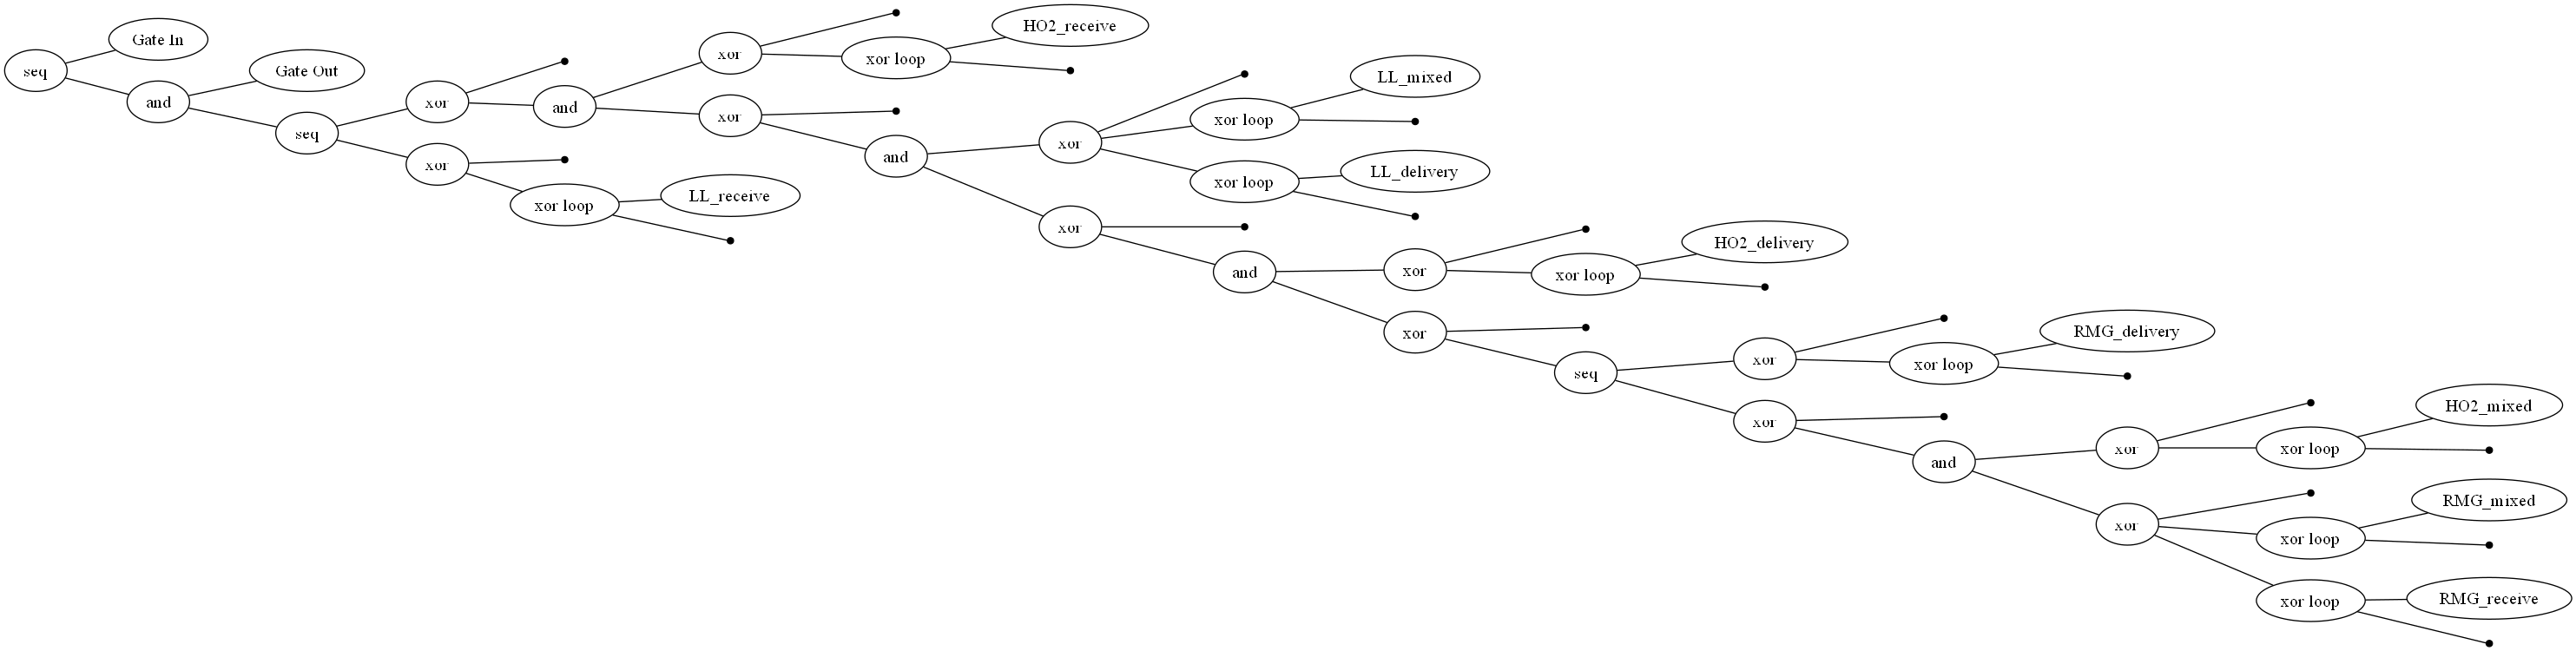
\includegraphics[width=\linewidth]{figures/discovery/process_tree.png}
    \subcaption{Process tree.}
    \label{fig:model_tree_theory}
\end{minipage}
\hfill
\begin{minipage}[t]{0.48\textwidth}
    \centering
    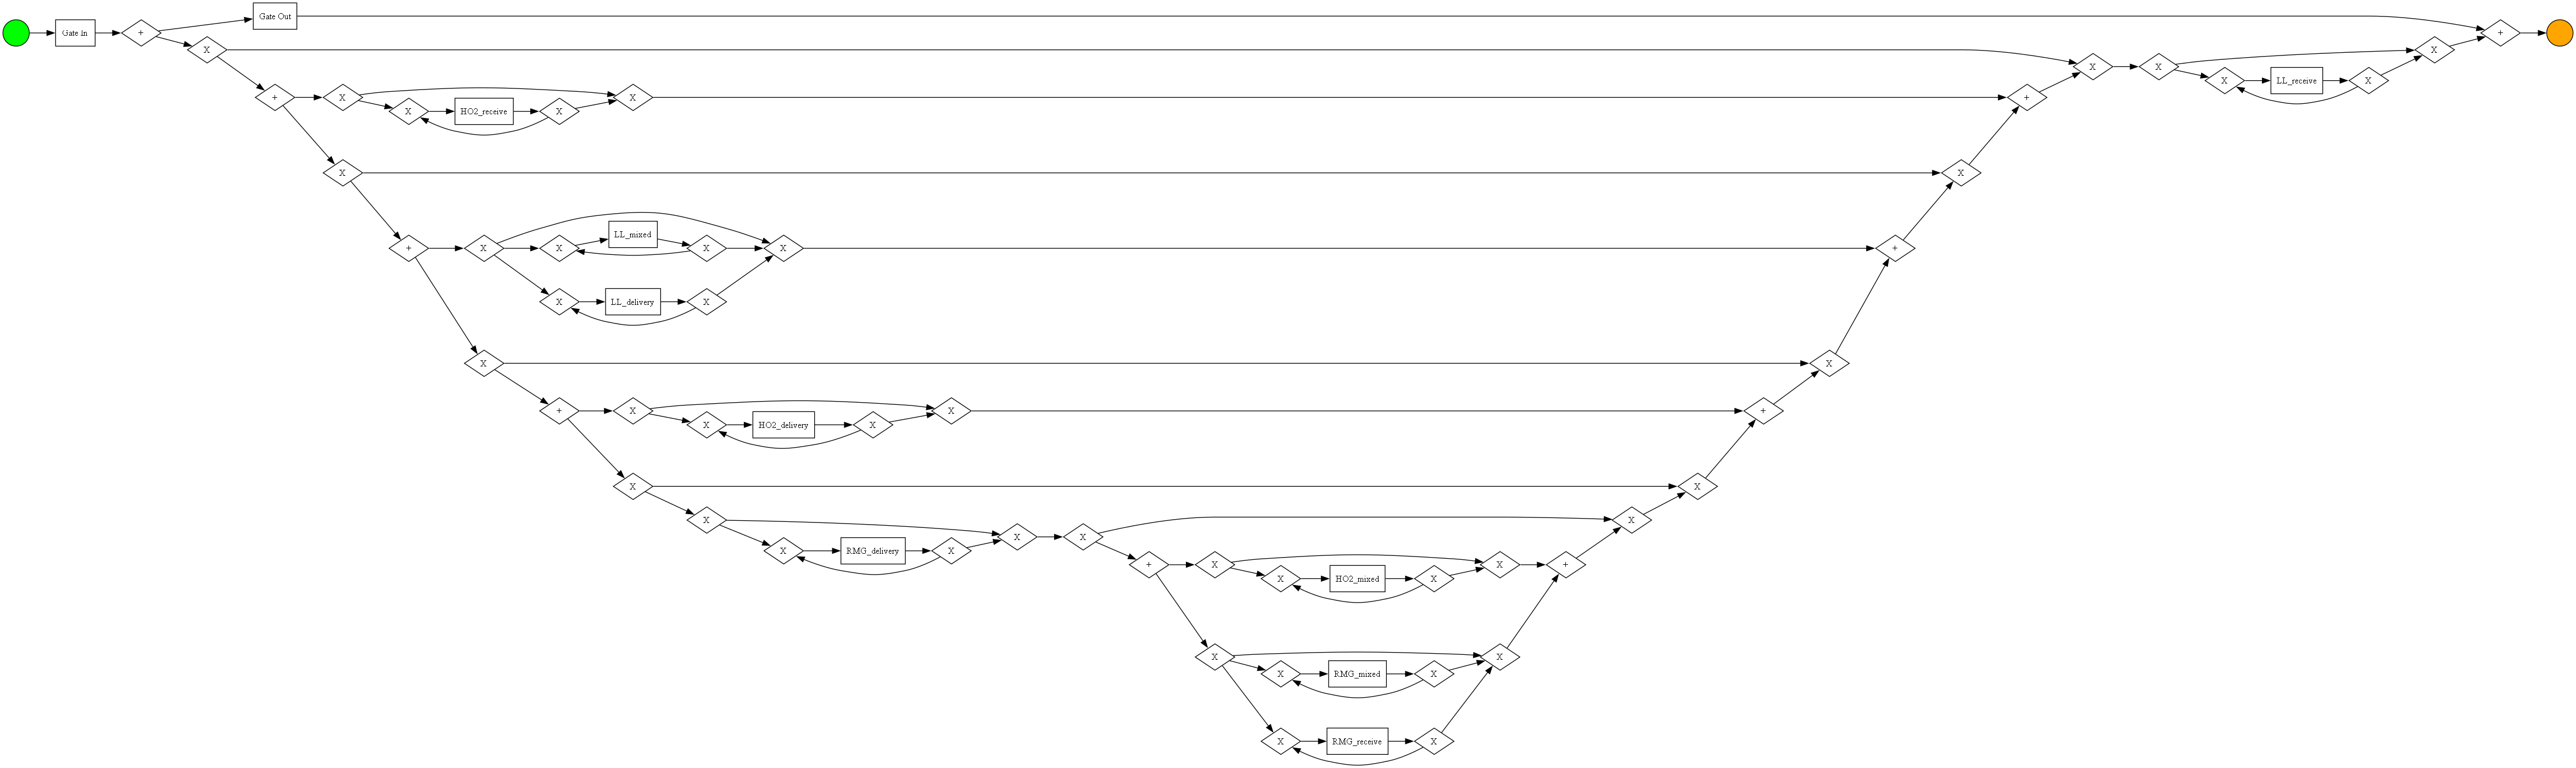
\includegraphics[width=\linewidth]{figures/discovery/bpmn.png}
    \subcaption{BPMN translation of the same process tree.}
    \label{fig:model_bpmn_theory}
\end{minipage}
\caption{Two representations of the same discovered control flow
(inductive miner on the CTB training log). The process tree exposes
the hierarchical operator structure; the BPMN translation preserves
the same behavior using the industry-standard graphical vocabulary.
Both models describe an identical set of allowed traces and are used
interchangeably in the process mining literature
\cite{PMvanDerAalst2016}.}
\label{fig:model_representations}
\end{figure}

\subsubsection{Conformance Checking}
While process discovery focuses on constructing process models, conformance checking focuses on comparing observed process executions with an existing process model \cite{aalst2012ConformanceChecking}. The objective is to identify deviations between the discovered model and the observed reality. Resulting deviations can indicate compliance violations, process inefficiencies, exceptional cases, or outdated process documentation. The quality of discovered process models is commonly evaluated using four criterias \cite{aalst2012ConformanceChecking,PMvanDerAalst2016}: 

\begin{itemize} \item \textbf{Fitness}: 
Measures how well the process model can reproduce the observed behavior in the event log. A model with high fitness allows most observed traces to be replayed without deviations.
\item \textbf{Precision}:
Measures how much additional behavior the model allows beyond the behavior observed in the event log. A precise model avoids allowing many unrealistic or unobserved execution paths. 
\item \textbf{Generalization}: 
Measures whether the model captures the underlying process behavior rather than only reproducing the exact traces contained in the event log. A model should therefore allow plausible behavior that was not necessarily observed in the available sample. 
\item \textbf{Simplicity}: 
Measures the complexity of the process model. Among models that describe the observed behavior sufficiently well, simpler models with fewer unnecessary elements and relations are generally preferred because they are easier to be interpreted and analysed. 
\end{itemize}

These criteria provide a balanced framework for evaluating process model quality and form the basis of many process-mining evaluation approaches. 

\paragraph{A*-based optimal alignment.}
\label{sec:astar_alignment_definition}
An alignment relates an observed trace to an executable run of a process
model. Formally, it is a sequence of three move types: a
\emph{synchronous move} consumes an event and fires a transition with the
same visible label; a \emph{log move} consumes an event without a
corresponding model transition; and a \emph{model move} fires a model
transition without consuming an observed event. A cost function normally
assigns zero cost to synchronous moves and positive, configurable costs
to deviations. An optimal alignment $\lambda^{\star}$ is therefore
\begin{equation}
\lambda^{\star}=\arg\min_{\lambda\in\Lambda(\sigma,N)} c(\lambda),
\end{equation}
where $\Lambda(\sigma,N)$ is the set of legal alignments between trace
$\sigma$ and process model $N$ \cite{aalst2012ConformanceChecking,
Adriansyah2011CostFitness}.

The qualifier ``A*-based'' refers to the search procedure, not to a
different kind of alignment. A* explores the product state space of the
current trace position and the current model state (for a Petri net, its
marking). It orders candidates by $f=g+h$, where $g$ is accumulated move
cost and $h$ is an admissible lower bound on the remaining cost. With an
admissible heuristic, the first complete solution is cost-optimal
\cite{Adriansyah2011CostFitness}. The resulting event--transition
correspondence supports conformance diagnostics and timestamp replay for
performance analysis \cite{aalst2012ConformanceChecking}; it does not
turn a model-derived enablement instant into an independently observed
timestamp.

\subsubsection{Process Enhancement} The Process Mining literature distinguishes three major categories of process mining techniques: process discovery, conformance checking, and process enhancement \cite{PMvanDerAalst2016}. The discovery creates a process model from event logs, conformance checking compares observed behavior with existing models and process enhancement then aims to improve existing process models using information extracted from event data. Enhancement includes different approaches. For example, performance information such as waiting times or activity durations can be projected onto a process model. Resource assignments, bottlenecks, and workload information can be incorporated to create richer process representations. Process enhancement can therefore enable process responsibles not only to understand how processes operate, but also identify opportunities for process improvement and optimization \cite{PMvanDerAalst2016}.

%%%%%%%%%%%%%%%%%%%%%%%%%%%%%%%%%%%%%%%%%%%%%%%%%%%%%%%%%%%%%%%%%%%%%% 
\section{Business Process Simulation} %%%%%%%%%%%%%%%%%%%%%%%%%%%%%%%%%%%%%%%%%%%%%%%%%%%%%%%%%%%%%%%%%%%%%% 

\subsection{Fundamentals of Business Process Simulation} 
Business Process Simulation (BPS) is an established analytical technique used to reproduce and analyze the dynamic behavior of business processes within a virtual environment. Rather than having to experiment directly on operational systems, organizations can build executable models that represent required process characteristics and repeatedly execute these models under controlled conditions. This allows process behavior to be observed without disturbing live operations \cite{BPSAalst2015}. Van der Aalst defines simulation as a flexible approach for analysing business processes and evaluating alternative operational scenarios. By recreating process executions under varying conditions, simulation can estimate process performance indicators such as throughput times, waiting times, resource utilization, service levels, and operational costs before changes have to be implemented in practice \cite{BPSAalst2015}. The primary purpose of simulation is the decision support. Business processes often run under uncertainty, dynamic resource interactions, and complex dependencies that make standard analytical evaluation difficult. Simulation provides a safe and cost-efficient environment for assessing operational modifications, while avoiding all the risks associated with real-world experimentation \cite{BPSAalst2015}. One of the most important applications of simulation is the so called \textit{what-if analysis}. What-if analyses evaluate how process performance changes under alternating assumptions or operational configurations. Typical examples include increasing the number of available resources, modifying routing rules, changing workload levels, or introducing new operational policies. By comparing simulation outcomes from different scenarios, decision makers can assess the expected consequences of proposed changes before implementation \cite{BPSAalst2015}. Because of its ability to represent dynamic process behavior and operational dependencies, simulation has become an established decision-support tool in fields such as manufacturing, healthcare, logistics, supply-chain management, and business process management. More recently, Process Mining research has increasingly integrated simulation based on observed event data, enabling simulation models to be discovered and calibrated directly from recorded process executions \cite{PMRozinat2009,Camargo2020}. 

\subsection{Business Process Simulation Models} 
A simulation model serves as a simplified representation of a real-world process. Although modeling approaches can vary, most business process simulation models consist of several fundamental perspectives that determine process behavior during simulation runs \cite{BPSAalst2015,PMRozinat2009}. 

\subsubsection*{Control Flow} 
The control-flow perspective describes the general behavioral structure of the process. It determines which activities exist, in which order they may occur, and which alternative execution paths are possible. In simulation models, the control-flow model serves as the structural backbone that governs the process execution. Commonly used representations include Petri nets, BPMN models, process trees, and workflow graphs \cite{PMvanDerAalst2016,BPSAalst2015}. 

\subsubsection*{Arrival Process} 
The arrival process defines how new process instances enter the system. In business processes, this typically corresponds to customer requests, orders, applications, service tickets, or other incoming work items. Arrival behavior is commonly represented through statistical distributions that describe the time between consecutive process initiations or arrivals. Since the incoming workload levels directly influence waiting times and resource utilization, realistic arrival modeling is essential for acurate simulation results \cite{BPSAalst2015,PMRozinat2009}. 

\subsubsection*{Resources} 
Resources represent the entities that execute process activities. Depending on the application domain, resources may correspond to employees, machines, vehicles, cranes or other terminal equipment. Resource models typically include information about availability, capacities, execution capabilities and multitasking abilities, working schedules, and allocation policies. Resource constraints are often important determinants of process performance because multiple process instances compete for limited resource capacity \cite{BPSAalst2015}. 

\subsubsection*{Activity Durations} 
The timing perspective describes how long activities require for their execution. Typical simulation models distinguish between processing times, waiting times, and overall case durations. Activity durations can be represented through probability distributions derived from historical observations. These temporal characteristics largely determine process performance and throughput behavior \cite{BPSAalst2015,PMRozinat2009}. 

\subsubsection*{Decision Logic} 
Business processes usually contain decision points where alternative execution paths can be selected. A Models learned decision logic determines how these routing decisions are made during simulation. Traditional simulation models employ static branching probabilities that specify how often a particular path is chosen. More advanced approaches model decisions as functions of contextual information, process attributes, or operational conditions at certain points in the path \cite{PMRozinat2009,mannhardt2023stochasticProcessesModelling}. 
\begin{sloppypar}
Together, control flow, arrivals, resources, timing information, and decision logic define the behavior of a simulation model. These perspectives form the foundation of both traditional manually developed simulation models and modern simulation-discovery approaches discussed later in this chapter. 
\end{sloppypar}


\subsection{Simulation-Based Decision Support} 
Container terminals operate in very dynamic environments characterized by fluctuating demand, limited resource capacity, and strong interdependencies between operational processes. Managers must continuously make decisions regarding equipment allocation, workforce planning, storage relocation strategies, truck appointment policies, and capacity utilization while maintaining uninterrupted terminal operations. Direct experimentation in a live terminal environment is often impractical because operational changes may negatively affect service quality, throughput, or customer satisfaction. As a consequence, simulation has become one of the most widely applied decision-support approaches in container terminal research \cite{Bruzzone2012,Kastner2021,Carboni2025}. By providing a virtual representation of terminal operations, simulation enables decision makers to evaluate operational alternatives before implementation. Typical applications include: 

\begin{itemize} 
    \item evaluation of truck appointment policies, 
    \item resource and workforce planning, 
    \item capacity planning and investment decisions, 
    \item yard layout and storage strategies, 
    \item yard crane allocation policies, 
    \item congestion analysis and bottleneck identification, 
    \item equipment scheduling and maintenance planning. 
\end{itemize} 

A core advantage of simulation is its ability to support what-if analyses. Alternative operational scenarios can be evaluated under identical conditions, allowing direct comparison of performance measures such as truck turnaround times, resource utilization, throughput, waiting times, and service levels. This capability is particularly valuable in container terminals because small operational changes frequently generate system-wide effects due to the strong interdependencies between gate operations, yard processes, and vessel handling activities \cite{CTSteenken2004,Bruzzone2012,Kastner2021}. For truck operations, simulation has been extensively applied to study the effects of Truck Appointment Systems (TAS), gate capacities, yard utilization, and equipment allocation strategies. Such analyses are usually terminal specific, but can support terminal operators in balancing efficiency improvements with operational robustness under uncertain workloads and changing operating conditions \cite{Bett2024,CTprocessMiningTAS2020}. 

\subsection{Simulation Model Calibration}
Calibration estimates or adjusts simulation parameters so that the
model represents the observed operating conditions. Typical tasks
include fitting arrival and duration distributions, estimating resource
capacities, and learning routing probabilities or context-dependent
decision rules from historical observations
\cite{PMRozinat2009,Camargo2020}. In simulation discovery, many of these
steps form part of the automated discovery procedure itself. Calibration
must nevertheless be distinguished from validation: agreement with the
data used to fit a model demonstrates in-sample fit, whereas an
independent assessment requires data that did not determine those
parameters. Section~\ref{sec:simulation_validation_background} develops
the corresponding verification and validation concepts.


%%%%%%%%%%%%%%%%%%%%%%%%%%%%%%%%%%%%%%%%%%%%%%%%%%%%%%%%%%%%%%%%%%%%%%%%%%%%%%%%%
\section{Simulation Discovery and Data-Aware Simulation} 
%%%%%%%%%%%%%%%%%%%%%%%%%%%%%%%%%%%%%%%%%%%%%%%%%%%%%%%%%%%%%%%%%%%%%%%%%%%%%%%%%

The previous sections established the main components of Business Process Simulation and the role of event logs in Process Mining. Simulation discovery connects these two perspectives by deriving executable simulation behavior directly from recorded process executions. Rather than introducing simulation parameters as manually specified assumptions, simulation-discovery approaches estimate them from event logs and integrate them into an executable process model \cite{PMRozinat2009,Camargo2020,simod2024}. The development of this research stream has progressively moved from the discovery of classical stochastic simulation parameters toward context-dependent and data-aware process behavior.

\subsection{From Simulation Discovery to Data-Driven Simulation} 

One of the foundational approaches to automatically derive simulation models from event logs was proposed by Rozinat et al. \cite{PMRozinat2009}. Their framework combines Process Mining and simulation by extracting several behavioral perspectives from historical executions, including control flow, temporal behavior, resource assignments, arrival characteristics, and routing probabilities.

Subsequent research extended this idea by refining the stochastic representation of process behavior. Solti et al. \cite{stochastikPetriNets2013Solti} investigate the discovery of stochastic Petri nets with arbitrary delay distributions, thereby integrating richer temporal behavior into formally discovered process models. Later, Camargo et al. \cite{Camargo2020} proposed a more automated framework for discovering executable Business Process Simulation models from event logs, including process structure, activity durations, resource pools, calendars, and arrival behavior. More recent frameworks such as Simod further systematise the automated discovery and calibration of simulation models from event data \cite{simod2024}.

A parallel branch researches uprising expressive generative models of process behavior. Camargo et al. \cite{Camargo2021} compare conventional data-driven process simulation with deep-learning-based generative models, illustrating that simulation discovery can move beyond separately fitted marginal distributions and toward models capable of learning more complex behavioral dependencies. This increased expressiveness, but at the same time also raises questions about transparency and configurability, which are discussed in Section~\ref{sec:explainable_simulation}.

The development can therefore be understood as a shift from extracting conventional simulation parameters from event logs towards learning increasingly enabled stochastic relationships between process state and simulated behavior \cite{PMRozinat2009,Camargo2020,Camargo2021}.


\subsection{Discovery of Simulation behavior} 

The simulation perspectives introduced in Section~\ref{sec:bps_models} remain the core objects of discovery, but the way they are represented has evolved considerably.

\subsubsection{Control-Flow and Stochastic Routing}

Early simulation-discovery approaches combined process discovery with stochastic information derived from observed executions \cite{PMRozinat2009}. While a discovered process model determines which activities may occur, stochastic weights determine how likely alternative paths actually are. Stochastic process discovery therefore extends purely structural process models with estimating the relative likelihood of alternative transitions \cite{stochastikPetriNets2013Solti,burke2020stochasticPD}.

The quality of the discovered control-flow structure stays important for simulation because the model defines the behavior that can be generated. Excessive generalisation may enable execution paths that were not observed or that are operationally implausible, whereas overly restrictive models may fail to represent legitimate process variability \cite{PMvanDerAalst2016,VinciDeLeoni2025Repair}. The balance between fitness and precision is therefore not only relevant for process discovery but also directly affects the behavioral space of the resulting simulator \cite{VinciDeLeoni2025Repair}.

\subsubsection{Temporal and Resource Behavior}

Simulation-discovery research has progressively moved from globally fitted distributions toward more differentiated temporal and resource models. Early approaches estimate execution times, waiting behavior, and resource characteristics from observed event-log distributions \cite{PMRozinat2009,stochastikPetriNets2013Solti}. More recent approaches additionally represent calendars, resource pools, allocation rules and heterogeneous resource behavior \cite{Camargo2020,BPSdifferentiatedResources2022}.

This development is particularly relevant because temporal behavior is rarely independent of the operational context. Execution and waiting times may vary with workload, resource availability, case characteristics or previous process behavior. Similarly, the probability of selecting a particular resource may depend on more than a static activity-resource mapping \cite{BPSdifferentiatedResources2022,Vinci2026prosit}. Recent simulation-discovery approaches therefore increasingly model these dimensions conditionally rather than as one global distribution per activity or resource.

\subsubsection{Arrival behavior}

Arrival processes have likewise evolved from globally fitted inter-arrival distributions toward context-dependent representations. Classical simulation-discovery approaches estimate inter-arrival times from historical case-start timestamps \cite{PMRozinat2009,Camargo2020}. More recent approaches can condition arrival behavior on temporal or contextual information, allowing the simulator to represent non-stationary workload patterns rather than assuming a single pooled arrival process \cite{Vinci2026prosit}. This distinction is important in operational settings where demand varies systematically across hours, weekdays, or operating periods.


\subsection{Data-Aware and Process-State-Aware Simulation}

A central limitation of classical stochastic simulation models is that routing probabilities and other behavioral parameters are often estimated globally. For example, if two alternative process paths occur with frequencies of 70\,\% and 30\,\%, a conventional stochastic model may assign these probabilities independently of the characteristics of the particular case. Such a representation captures how often alternatives occurred, but not why different process instances followed different paths \cite{PMRozinat2009,burke2020stochasticPD}.

Data-aware simulation addresses this limitation by conditioning stochastic behavior on process data. Mannhardt et al. \cite{mannhardt2023stochasticProcessesModelling} extend stochastic Petri nets with data-dependent transition weights, so that the probability of an enabled transition can depend on process variables instead of being represented by one global value. The resulting model therefore captures systematic differences between cases with different characteristics.

De Leoni et al. \cite{Vinci2023Inf.Activ.Prob} extend this idea through the concept of the \textit{process state}. Rather than conditioning decisions only on static case attributes, the process state may also describe information accumulated during the execution of the case, including process-variable values and the history of previously executed activities. Their results show that incorporating this richer representation of the current process state can improve the estimation of activity-firing probabilities compared with basic frequency-based branching probabilities.

The conceptual development can therefore be represented as:

\begin{center}
Static Branching Probabilities \\
$\downarrow$ \\
Stochastic Process Models \\
$\downarrow$ \\
Data-Dependent behavior \\
$\downarrow$ \\
Process-State-Aware Simulation
\end{center}

Recent work extends data awareness beyond routing behavior. López-Pintado et al. \cite{lopez2024} investigate the discovery and simulation of data-aware business processes more broadly, reflecting a shift toward simulation models in which multiple behavioral dimensions depend on process context rather than only on marginal historical frequencies.


\subsection{ProSiT as a Probabilistic Data-Aware Simulation Framework}

The ProSiT framework represents a recent development within this research direction \cite{Vinci2026prosit}. Instead of applying data awareness only to routing decisions, ProSiT models several simulation dimensions through probabilistic white-box predictors, including control-flow decisions, execution times, waiting times, resource selection, and arrival behavior.

The framework uses probabilistic decision trees to partition the available feature space and associates each resulting leaf with a local probability distribution. Simulation behavior can therefore differ between process contexts while remaining stochastic. This is conceptually different from both a conventional simulation model with one global distribution per parameter and a deterministic predictive model that returns a single point estimate.

An important distinction is required between different forms of contextual information. In the published ProSiT framework, simulation-parameter discovery can use trace attributes, execution history, resource information, temporal information, and workload-related features \cite{Vinci2026prosit}. This does not imply unrestricted support for arbitrary event-level attributes that change continuously during execution. The more general process-state perspective described by Mannhardt et al. \cite{mannhardt2023stochasticProcessesModelling} and de Leoni et al. \cite{Vinci2023Inf.Activ.Prob} therefore provides a broader conceptual framework than the particular feature representation currently implemented in ProSiT.

For this thesis, ProSiT is particularly useful because its level of contextual conditioning can be varied experimentally. The framework therefore makes it possible to test whether increasing model expressiveness actually translates into improved held-out simulation fidelity in the CTB truck process.


\paragraph{Configurable expressiveness in ProSiT.}

Two ProSiT configuration parameters are particularly relevant for the experimental design in Section~\ref{sec:simulation_discovery_methodology} \cite{Vinci2026prosit}:

\begin{itemize}
    \item \texttt{max\_depth\_tree} controls the maximum depth of the probabilistic decision trees used for conditional simulation behavior. Setting \texttt{max\_depth\_tree}$=0$ disables conditional tree-based modelling and yields an unconditional distribution-based configuration. Increasing the depth allows the model to distinguish more detailed combinations of contextual features, while also increasing model complexity and potential overfitting.

    \item \texttt{use\_workload\_features} determines whether workload-related features are made available to the waiting-time and resource-selection models. When enabled, these models can condition their behavior on the current operational workload and queue state in addition to the remaining contextual attributes.
\end{itemize}

These parameters define the comparison used later in this thesis between a distribution-based configuration, a data-aware configuration, and a data-aware configuration additionally enriched with workload information. Whether this increased expressiveness improves simulation fidelity is treated as an empirical question rather than assumed in advance.

%%%%%%%%%%%%%%%%%%%%%%%%%%%%%%%%%%%%%%%%%%%%%%%%%%%%%%%%%%%%%%%%%%%%%%%%%%%%%%%%%
\section{Explainable and White-Box Simulation}
%%%%%%%%%%%%%%%%%%%%%%%%%%%%%%%%%%%%%%%%%%%%%%%%%%%%%%%%%%%%%%%%%%%%%%%%%%%%%%%%%%

\subsection{Explainability in Simulation-Based Decision Support}
Business Process Simulation is becoming increasingly popular to support operational and strategic decision making. Simulation results are often the basis for resource-allocation strategies ans decisions, process redesign initiatives, capacity planning, and investment evaluations. Therefore decision makers have to be able to understand why a simulation model produces a particular outcome and how simulation behavior changes when process parameters are modified. Traditional Business Process Simulation models are transparent from design \cite{BPSAalst2015}. Their control-flow structures, routing probabilities, resource allocations, and time assumptions are manually specified and can therefore be analysed and modified by developers and domain experts. That way, simulation users can directly understand the assumptions underlying the generated simulation results \cite{BPSAalst2015}. Recent advances in simulation discovery increasingly employ machine-learning and deep-learning techniques to improve the simulation accuracy. These approaches learn behavioral patterns directly from historical event data and often outperform manually calibrated models in terms of predictive capabilities \cite{Camargo2020, Camargo2021}. However, the resulting models frequently behave as black-box systems. While they can generate more accurate predictions, the internal decision mechanisms that govern the simulation behavior, are not readily interpretable by developers or human analysts. This creates a tension between predictive accuracy and explainability. Black-box simulation models therefore may successfully reproduce historical process behavior while simultaneously limiting the analyst's ability to understand why particular routing decisions, waiting times, or resource allocations are generated. Consequently, the simulation model becomes difficult to inspect, configure, validate, and trust for operational decision support \cite{runtimeIntegration2024}. The explainability problem becomes especially relevant for what-if analyses. Business Process Simulation is not only intended to reproduce observed behavior but also to evaluate hypothetical future scenarios. Devlopers have to be able to intentionally modify process parameters, resource settings or decision rules. In black-box simulation approaches, the underlying behavioral logic is often inaccessible, making it difficult to assess whether the simulated reactions to process changes are realistic and trustworthy \cite{runtimeIntegration2024}. To address these limitations, recent research has started investigating explainable simulation models that combine the predictive capabilities of machine-learning approaches with transparent and interpretable decision logic. The goal is not only to reproduce process behavior accurately but also to expose the reasoning mechanisms that determine simulation outcomes. Explainability therefore becomes an important prerequisite for trustworthiness, configurability, and practical adoption of data-driven simulation models.

\subsection{Probabilistic White-Box Simulation Models} 
The concept of white-box simulation emerged as a response to the increasing reliance on opaque machine-learning models for simulation parameter discovery. White-box simulation models aim to make behavioral decisions explicitly visible and interpretable while maintaining a high degree of simulation accuracy. A key motivation behind white-box simulation is that business analysts must be able to inspect, understand, and modify the simulation behavior that drives decision-support outcomes. Unlike black-box predictors, white-box approaches expose the discovered decision rules and allow analysts to evaluate the causal relationships that influence simulation parameters. An important step towards explainable simulation is represented by the Runtime Integration of Machine Learning and Simulation (RIMS) framework proposed by Meneghello et al. \cite{runtimeIntegration2024}. RIMS combines traditional discrete-event simulation with predictive machine-learning models at runtime. The authors explicitly argue that purely deep-learning-based simulation approaches suffer from limited explainability and restricted support for what-if analyses. By maintaining an explicit simulation model while integrating learned predictions during execution, RIMS seeks to combine simulation transparency with data-driven prediction capabilities \cite{runtimeIntegration2024}. More recently, Vinci et al. introduced the ProSiT framework (\textit{PROcess SImulation Tool}), which represents one of the first dedicated white-box simulation-discovery approaches \cite{Vinci2026prosit}. ProSiT extends data-aware simulation discovery by replacing opaque prediction mechanisms with probabilistic decision trees. These trees are used to represent multiple simulation dimensions including: \begin{itemize} \item control-flow decisions, \item activity execution times, \item waiting times, \item resource assignment behavior, \item arrival processes. \end{itemize} The central idea of ProSiT is that simulation behavior should remain directly interpretable. Instead of producing predictions through hidden neural-network representations, behavioral rules are exposed explicitly in the form of decision-tree structures. Analysts can therefore inspect, understand, and modify the conditions influencing simulation behavior \cite{Vinci2026prosit}. An additional contribution of ProSiT is the integration of uncertainty through probabilistic decision trees. Traditional decision trees often generate deterministic predictions. In contrast, probabilistic decision trees capture distributions of possible outcomes and thereby preserve the stochastic nature required for realistic process simulation \cite{Vinci2026prosit}. This is particularly important because simulation models aim not only to reproduce average behavior but also the variability observed in real operational environments. Experimental evaluations presented by Vinci et al. indicate that probabilistic white-box models can achieve simulation accuracy comparable to, and in some cases exceeding, alternative black-box approaches while simultaneously improving interpretability and configurability \cite{Vinci2026prosit}. Furthermore, the framework enables process analysts to directly edit discovered rules and evaluate modified decision scenarios without retraining complex machine-learning models. Despite these promising results, research on white-box simulation remains at an early stage. Current evidence is largely limited to benchmark datasets and business-process environments investigated by the authors themselves. Large-scale empirical evaluations across different domains remain scarce. In particular, little evidence currently exists regarding the behavior of white-box simulation models in highly dynamic cyber-physical systems such as container terminals. Moreover, explainability itself remains difficult to quantify. While decision trees are generally considered more transparent than neural networks, there is currently no universally accepted framework for measuring the practical interpretability of simulation-discovery models. Existing evaluations primarily focus on simulation accuracy, leaving questions related to user trust, decision-support quality, and operational usefulness largely unexplored. Consequently, white-box simulation should not yet be regarded as a mature solution to the explainability challenge. Rather, it represents an emerging research direction that attempts to balance three competing objectives: 

\begin{enumerate} 
\item simulation accuracy, 
\item simulation explainability, 
\item simulation configurability. 
\end{enumerate} 

The ProSiT framework currently represents one of the most comprehensive realizations of this vision and serves as the methodological foundation for the simulation approach investigated in this thesis \cite{Vinci2026prosit}.

%%%%%%%%%%%%%%%%%%%%%%%%%%%%%%%%%%%%%%%%%%%%%%%%%%%%%%%%%%%%%%%%%%%%%%%%%%%%%%%%%%%
For terminological precision, the relationships exposed by such learned
rules are statistical associations conditional on the training data and
model specification. Their visibility supports inspection and deliberate
configuration, but does not by itself establish causal effects.

%%%%%%%%%%%%%%%%%%%%%%%%%%%%%%%%%%%%%%%%%%%%%%%%%%%%%%%%%%%%%%%%%%%%%%%%%%%%%%%%%%%
\section{Simulation Verification, Validation, and Trustworthiness}
\label{sec:simulation_validation_background}
The central validation question is not whether a simulator is merely
executable, but whether it is sufficiently credible for its intended
use. This qualification is essential: a model may be adequate for
reproducing historical truck turnaround distributions while remaining
inadequate for predicting the effect of an intervention outside the
range of the observed data \cite{Sargent2013Validation,BPSAalst2015}.
Automatically discovered simulation models do not remove this
requirement. They replace some manual assumptions with assumptions about
event-log semantics, discovery algorithms, data attributes and fitted
distributions, all of which require examination.

\subsection{Foundational Distinction Between Verification and Validation}

Sargent separates several questions that are often conflated under the
single term \emph{validation} \cite{Sargent2013Validation}.
\emph{Conceptual-model validity} asks whether the theories, assumptions
and logical relationships in the conceptual model are reasonable for
the intended purpose. \emph{Computerized-model verification} asks
whether that conceptual model has been implemented correctly.
\emph{Data validity} concerns whether the data used to construct,
calibrate and evaluate the model are adequate. Finally,
\emph{operational validity} asks whether the computerized model's
output behaviour is sufficiently accurate over the domain in which the
model is intended to be used. Historical-data validation---running the
model under historical input conditions and comparing its output with
observed system data---is one technique for assessing operational
validity \cite{Sargent2013Validation}.

Table~\ref{tab:validation_evidence_types} maps these distinctions to the
type of evidence needed in an automatically discovered BPS study. The
categories are complementary rather than interchangeable. For example,
a low event-log distance is evidence of operational fidelity, but it
cannot show that a timestamp proxy has the correct physical meaning or
that the simulator implemented a resource constraint as intended.

\begin{table}[htbp]
\centering
\caption{Validation questions and corresponding evidence in an
event-log-discovered simulation study, based on Sargent's framework
\cite{Sargent2013Validation}.}
\label{tab:validation_evidence_types}
\begin{tabular}{p{0.23\textwidth}p{0.29\textwidth}p{0.39\textwidth}}
\toprule
\textbf{Question} & \textbf{Validity concept} & \textbf{Typical evidence} \\
\midrule
Is the abstraction defensible? & Conceptual-model validity &
Domain review of case boundaries, event semantics, resource meanings
and physical constraints \\
Was the abstraction implemented correctly? & Computerized-model
verification & Unit and integration tests, structural contracts,
reproducible seeds and parameter-provenance checks \\
Are discovery and evaluation data suitable? & Data validity &
Event-log quality checks, timestamp semantics, leakage prevention and a
training/test separation \\
Does the model reproduce observed behaviour? & Operational validity &
Comparison of simulated and held-out real logs across multiple process
perspectives and stochastic replications \\
Does a scenario predict the true intervention effect? & Predictive
validity outside the historical regime & Intervention observations,
controlled field evidence or additional domain-supported sensitivity
analysis \\
\bottomrule
\end{tabular}
\end{table}

This distinction also clarifies the scope of this thesis. The
real-versus-simulated event-log comparison is a form of held-out
historical-data or operational validation. The event-log construction
and the physical RMG capacity constraint contribute data- and
conceptual-validity evidence, while executable case contracts and
provenance checks contribute verification evidence. None of these alone
proves that every what-if response is the true causal response of the
terminal.

\subsection{From Historical Logs to Operational Validation}

Process Mining provides a natural representation for historical-data
validation because both the observed system and the simulator can be
represented by event logs. Rozinat et al. established an early version
of this principle: they discover control-flow, data, performance and
resource perspectives, integrate them into a coloured Petri-net
simulation model, simulate a second event log, and analyse how well that
generated log approximates the characteristics of the original log
\cite{PMRozinat2009}. This is stronger than checking whether the
discovered model can execute; it evaluates whether its generated
behaviour resembles recorded behaviour.

Camargo et al. formalise the same idea as an optimisation objective.
Candidate BPS configurations generate event logs and hyperparameter
optimisation searches for the configuration that maximises similarity
to observed log behaviour \cite{Camargo2020}. Their later comparison of
data-driven simulation and deep generative models further demonstrates
why quality must not be inferred from trace frequencies alone:
conventional data-driven simulators may reproduce activity sequences
and their frequencies while performing worse on temporal dynamics
\cite{Camargo2021}.

The implication is that operational fidelity is multi-dimensional.
Relevant perspectives include control flow, activity and case timing,
case arrivals, congestion and resource behaviour. A model can be close
to the real log in one perspective and far away in another; collapsing
all discrepancies into one number can therefore hide the mechanism
that is incorrectly represented
\cite{ChapelaCampa2023Trust,Chapela2025SimQuality}.

\subsection{Multi-Perspective Event-Log Comparison}

Chapela-Campa et al. provide the validation framework that most closely
matches the evaluation problem of this thesis
\cite{ChapelaCampa2023Trust,Chapela2025SimQuality}. Their starting point
is that the true BPS model is normally unavailable and that different
simulation engines use incomparable internal formats. They therefore
evaluate a model indirectly as a generator: multiple logs generated by
the BPS model are compared with an actual event log that was not used
to construct the model. The framework separates control-flow, temporal
and congestion perspectives and reports a measure for each instead of
claiming that one aggregate score represents overall model quality.
The measures are evaluated using controlled perturbations and by
comparing alternative automatically discovered BPS models, showing that
perspective-specific measures can identify the source of a discrepancy
\cite{Chapela2025SimQuality}.

\subsubsection{Control-Flow Perspective}

Control-flow output quality asks whether the simulator generates
activity sequences and sequence frequencies resembling the observed
process. It is distinct from replay fitness of a control-flow model:
fitness asks whether real traces are allowed by the model, whereas
output validation asks which traces the stochastic simulator actually
generates and with what frequency.

Stochastic conformance work applies transport distances to probability
distributions over traces or other behavioural abstractions
\cite{leeman2013EarthMovers}. Chapela-Campa et al. instead define two
simulation-oriented log distances \cite{ChapelaCampa2023Trust,
Chapela2025SimQuality}. Control-Flow Log Distance (CFLD) computes the
normalised Damerau--Levenshtein distance between trace pairs and uses
the Hungarian algorithm to find the minimum-cost one-to-one matching
between the two logs. CFLD therefore compares complete traces; it is not
merely a comparison of variant-frequency vectors. Because this matching
is computationally expensive, N-Gram Distance (NGD) compares normalised
frequencies of local activity subsequences. NGD is scalable and detects
local ordering differences, although it deliberately loses some
complete-trace information.

This thesis does not claim to implement the full Chapela-Campa metric
suite. Its structural evidence combines held-out Petri-net conformance,
explicit case-language contracts and yard-activity frequency error.
These measures answer the CTB-specific structural questions, while the
Chapela-Campa framework supplies the rationale for keeping structural
evidence separate from temporal fidelity.

\subsubsection{Temporal Perspective}

Identical or similar traces do not imply similar process performance.
Temporal validation considers whether the simulator reproduces when
events occur, how cases progress after arrival and how long activities
and complete cases take. Camargo et al. show empirically that a
generative model may represent control-flow frequencies adequately yet
miss temporal dynamics \cite{Camargo2021}.

The Chapela-Campa framework distinguishes three event-distribution
measures \cite{ChapelaCampa2023Trust,Chapela2025SimQuality}.
\emph{Absolute Event Distribution} (AED) compares event counts across
absolute calendar-time bins; \emph{Circadian Event Distribution} (CED)
compares recurring weekday and hour-of-day patterns; and
\emph{Relative Event Distribution} (RED) offsets timestamps by each
case's arrival and compares its temporal progression. Thus AED and RED
mean \emph{event distribution}, not absolute or relative error
distance. For end-to-end performance, Cycle Time Distribution (CTD)
compares the empirical distributions of complete case durations.

The CTB evaluation uses more directly interpretable distributions at
the level of its research questions: inter-arrival time, per-activity
yard service time, model-derived pre-service delay and case turnaround
time. Reporting complete distributions rather than only their means is
important because equal averages can conceal differences in dispersion,
skewness or tails. Per-activity results additionally prevent common RMG
events from concealing weaker fidelity for less frequent yard
activities.

\subsubsection{Arrival and Congestion Perspectives}

Congestion is a system-level consequence of the interaction between
demand, service requirements and resource availability. It cannot be
validated from activity-duration marginals alone. Chapela-Campa et al.
use Case Arrival Rate (CAR) to compare binned arrival counts and shapes,
and CTD to compare the second major congestion component, the length of
time cases remain in the system
\cite{ChapelaCampa2023Trust,Chapela2025SimQuality}. An arrival model can
therefore be temporally unrealistic even if it generates the correct
total number of cases.

This issue is central at CTB: truck demand determines competition for
yard resources, and simultaneous arrivals are meaningful consequences
of the minute-resolved source data. The evaluation consequently reports
inter-arrival distance, simultaneous-arrival share and arrivals per
elapsed hour alongside turnaround and yard-service distributions.
These measures do not directly observe a physical queue; they assess
whether the generated workload and its resulting temporal behaviour
match what the available event log can identify.

\subsubsection{Wasserstein Distance}

For two one-dimensional distributions $F$ and $G$ with finite first
moments, the first Wasserstein distance can be written as
\begin{equation}
    W_1(F,G)=\int_{-\infty}^{\infty}|F(x)-G(x)|\,\mathrm{d}x .
\end{equation}
It has the optimal-transport interpretation of the minimum cost of
moving probability mass from one distribution to the other. For
durations measured in minutes, $W_1$ is also expressed in minutes,
which gives the discrepancy an operational scale.

Earth Mover's Distance (EMD) is closely related, but the terms should
not be treated as universally interchangeable. In the formulation used
by Chapela-Campa et al., EMD may compare time series with unequal total
mass and penalise the creation of missing mass, whereas first
Wasserstein distance assumes equal normalised mass
\cite{ChapelaCampa2023Trust,Chapela2025SimQuality}. For empirical
probability distributions with unit mass, the formulations coincide.
In Process Mining, related transport distances have also been used for
stochastic conformance checking over behavioural distributions
\cite{leeman2013EarthMovers}. In this thesis, the term \emph{EMD} for
service, inter-arrival and turnaround samples denotes the
one-dimensional $W_1$ distance between empirical distributions.

\subsubsection{Kolmogorov--Smirnov Statistic}

The two-sample Kolmogorov--Smirnov (KS) statistic is the maximum
vertical difference between the empirical cumulative distribution
functions of the simulated and observed samples
\cite{Massey1951KS}:
\begin{equation}
    D_{n,m}=\sup_x
    \left|F_{n,\mathrm{sim}}(x)-F_{m,\mathrm{real}}(x)\right|.
\end{equation}
Unlike $W_1$, it is dimensionless and bounded by zero and one. The two
statistics are complementary: $W_1$ measures integrated displacement
on the operational scale, while KS reports the largest local CDF gap.
The KS statistic can be accompanied by a hypothesis-test $p$-value, but
that $p$-value answers a different question from practical fidelity.
With large event logs, small and operationally unimportant differences
can be statistically significant. The magnitude of the statistic and
the distributional plots must therefore be interpreted separately from
null-hypothesis rejection.

\subsubsection{Additional Requirements for Data-Aware Discovery}

A data-aware simulator conditions behaviour on case attributes, process
state or workload information rather than using only global
distributions and branching frequencies
\cite{Vinci2023Inf.Activ.Prob,lopez2024,Vinci2026prosit}. This adds a
validation layer. First, every predictor used at a simulated decision
point must be available at that point; attributes computed from a later
outcome create target leakage even if aggregate log similarity is high.
Second, discovery and model selection must be separated from the final
test log. Third, the generated log must satisfy process and domain
invariants that aggregate distances may overlook.

White-box rules help because their split conditions and leaf
distributions can be inspected and deliberately modified
\cite{Vinci2026prosit}. Interpretability, however, is not equivalent to
validity or causality. A readable rule may encode a spurious association,
and two differently specified models may reproduce the same marginal
distribution. Validation should therefore combine held-out output
fidelity with rule inspection, leakage checks, structural contracts,
domain constraints and sensitivity analysis. This is particularly
important for the CTB application, where timestamp fields are
operational proxies and a resource label does not necessarily denote a
physically interchangeable crane or storage position.

\subsubsection{Stochastic Replication and Confidence Intervals}

A BPS model is a stochastic generator. One fixed model can generate
many possible event logs, whereas the real test log is only one observed
realisation. A single simulated log therefore confounds model fidelity
with the random draws of that run. Chapela-Campa et al. address this
problem directly: they generate $K$ logs from $K$ simulation runs,
match their case count and start point to an actual test log that was
not used for model construction, compare every generated log with that
test log, and construct confidence intervals for each perspective-
specific distance \cite{ChapelaCampa2023Trust}. Their controlled
evaluation uses $K=10$ replications and reports means and 95\,\%
intervals.

This design is consistent with classical simulation-output analysis,
where independent replications with different random-number streams
provide observations for estimating a mean and its Monte-Carlo
uncertainty \cite{Law2015Simulation}. For replication-level values
$x_1,\ldots,x_N$, a two-sided Student-$t$ interval is
\begin{equation}
    \bar{x}\ \pm\
    t_{0.975,N-1}\frac{s}{\sqrt{N}},
\end{equation}
where $s$ is the sample standard deviation across replications.

The interpretation of this interval must remain narrow. Conditional on
one frozen discovered parameter bundle and one fixed real test log, it
quantifies the variability caused by simulation sampling. It does not
include event-log sampling uncertainty, input-distribution estimation
uncertainty, alternative discovery outcomes, measurement error or
uncertainty about the correctness of a what-if response. Those require
additional resampling, repeated discovery, sensitivity experiments or
external domain evidence. Chapter~\ref{chp:experiments_and_framework}
uses this conditional Monte-Carlo interpretation for its ten-seed
protocol.

\subsection{Trustworthiness and the Boundary of Historical Validation}

Historical fidelity is necessary for a simulator that claims to
represent an existing process, but it is not sufficient for unrestricted
decision support. Chapela-Campa et al. explicitly identify this limit:
comparison with an original event log assesses replication of the
\emph{as-is} process, not the accuracy of predictions after a process
change \cite{ChapelaCampa2023Trust,Chapela2025SimQuality}. Similarly,
Sargent's purpose-relative view implies that evidence collected in one
operating region cannot automatically validate use in another
\cite{Sargent2013Validation}.

Trustworthiness is therefore an evidence bundle rather than another
single metric. It includes data and conceptual validity, verified
implementation, held-out multi-perspective fidelity, reproducibility,
transparent assumptions, stochastic robustness, domain review and
clear limits on extrapolation. ProSiT contributes inspectable and
configurable probabilistic rules \cite{Vinci2026prosit}; recent applied
work shows how discovered simulation models can be connected to a real
resource-allocation problem \cite{Hospital2026Vinci}. These properties
make validation and scenario discussion more accessible, but neither
white-box structure nor a successful application substitutes for
intervention-specific evidence.

Accordingly, this thesis does not claim to solve the general
trustworthiness problem of simulation discovery. It contributes a
container-terminal case study: the model is tested against an unseen
historical period, across structural, temporal and arrival perspectives,
with repeated stochastic runs and explicit domain constraints. Scenario
results are interpreted as conditional consequences of the documented
model assumptions, not as experimentally established causal effects.

\subsection{Research Gap}

Container terminals represent highly dynamic and resource-constrained operational environments characterized by complex interactions between truck processes, yard operations, storage systems, and handling equipment. As a result, simulation has become one of the most widely used analytical methods for supporting operational decision making in container terminal management \cite{Bruzzone2012,Kastner2021,Carboni2025}. Despite this extensive use of simulation, most container terminal simulation models continue to be developed manually. Model construction, calibration, and maintenance require substantial modelling effort and domain expertise, limiting scalability and practical applicability in rapidly changing operational environments \cite{PMRozinat2009}. Simulation discovery addresses this limitation by automatically generating simulation models from event logs. Over the past decade, significant advances have been achieved in the discovery of simulation parameters, data-aware decision logic, and automated model construction \cite{Camargo2020,simod2024,Vinci2026prosit}. More recently, data-aware simulation approaches demonstrated that contextual information and process-state representations can substantially improve simulation accuracy compared to traditional branching probabilities \cite{mannhardt2023stochasticProcessesModelling,Vinci2023Inf.Activ.Prob}. In parallel, white-box simulation approaches such as ProSiT introduced interpretable probabilistic decision models that aim to improve transparency and configurability while maintaining strong predictive performance \cite{Vinci2026prosit}. However, existing empirical evaluations have primarily been conducted in healthcare, administrative, and generic business-process environments. To date, there is limited evidence regarding the applicability and behavior of simulation-discovery approaches within large-scale container terminal operations. Furthermore, the increasing complexity of data-aware and decision-aware simulation models raises unresolved questions concerning: \begin{itemize} \item the robustness of automatically discovered simulation models, \item their trustworthiness for operational decision support, \item their ability to reproduce congestion effects and workload dynamics, \item the practical value of white-box simulation in complex logistics environments. \end{itemize} This thesis does not aim to provide a general answer to these broader research challenges. Rather, it contributes an empirical case study within the context of truck-handling operations at the HHLA Container Terminal Burchardkai (CTB). By evaluating simulation-discovery approaches in a real-world container terminal environment, the thesis provides evidence regarding their applicability, strengths, and limitations in a domain that has received comparatively little attention within the existing simulation-discovery literature.
